\documentclass[11pt,a4paper]{article}
\usepackage[a4paper,top=24mm,bottom=25mm,left=26mm,right=26mm,headsep=9mm]{geometry}
\usepackage{fontspec}
\defaultfontfeatures{Ligatures=TeX}
\setmainfont{LibertinusSerif-Regular.otf}[BoldFont=LibertinusSerif-Bold.otf,ItalicFont=LibertinusSerif-Italic.otf,BoldItalicFont=LibertinusSerif-BoldItalic.otf]
\setsansfont{LibertinusSans-Regular.otf}[BoldFont=LibertinusSans-Bold.otf,ItalicFont=LibertinusSans-Italic.otf]
\setmonofont{Inconsolatazi4-Regular.otf}[BoldFont=Inconsolatazi4-Bold.otf,Scale=MatchLowercase,Ligatures=TeXOff,StylisticSet=3]
\usepackage{unicode-math}
\setmathfont{LibertinusMath-Regular.otf}
\usepackage{microtype}
\usepackage{xcolor}
\definecolor{accent}{HTML}{843C35}
\definecolor{muted}{HTML}{66685F}
\definecolor{rulecolor}{HTML}{D8D2C4}
\usepackage{graphicx,booktabs,longtable,array,calc}
\usepackage{amsmath}
\usepackage{titlesec,needspace,etoolbox}
\usepackage{enumitem}
\usepackage{caption}
\usepackage{fancyhdr}
\usepackage{xurl}
\usepackage[unicode=true,colorlinks=true,linkcolor=accent,urlcolor=accent,bookmarksopen=true,pdftitle={Fuga inversa — Analysis and process},pdfauthor={GPT-6 Astra agents; directed by chi-feng}]{hyperref}
\usepackage{bookmark}
\usepackage{newunicodechar}
\newunicodechar{♭}{\ensuremath{\flat}}
\newunicodechar{♯}{\ensuremath{\sharp}}
\newunicodechar{♮}{\ensuremath{\natural}}
\newunicodechar{−}{\ensuremath{-}}
\setcounter{secnumdepth}{0}
\titleformat{\section}{\normalfont\Large}{}{0pt}{}
\titleformat{\subsection}{\normalfont\sffamily\normalsize\color{accent}}{}{0pt}{}
\titlespacing*{\section}{0pt}{3.2ex plus .6ex}{1.4ex}
\titlespacing*{\subsection}{0pt}{2.7ex plus .5ex}{1.1ex}
\pretocmd{\section}{\Needspace{6\baselineskip}}{}{}
\pretocmd{\subsection}{\Needspace{5\baselineskip}}{}{}
\renewcommand{\figurename}{Example}
\captionsetup{font=small,labelfont=bf,justification=raggedright,singlelinecheck=false,skip=9pt}
\setlength{\parindent}{0pt}
\setlength{\parskip}{.55em}
\linespread{1.045}
\setlist[itemize]{leftmargin=1.1em,itemsep=.55em,topsep=.5em}
\renewcommand{\arraystretch}{1.17}
\setlength{\tabcolsep}{4pt}
\setlength{\LTpre}{12pt}
\setlength{\LTpost}{13pt}
\setlength{\emergencystretch}{2em}
\setlength{\headheight}{22pt}
\pagestyle{fancy}
\fancyhf{}
\fancyhead[L]{\small\itshape\color{muted}Fuga inversa}
\fancyhead[R]{\small\sffamily\color{muted}Analysis and process}
\fancyfoot[C]{\small\color{muted}\thepage}
\renewcommand{\headrulewidth}{.25pt}
\renewcommand{\headrule}{\hbox to\headwidth{\color{rulecolor}\leaders\hrule height \headrulewidth\hfill}}
\providecommand{\tightlist}{\setlength{\itemsep}{0pt}\setlength{\parskip}{0pt}}
\providecommand{\pandocbounded}[1]{#1}
\makeatletter
\def\maxwidth{\ifdim\Gin@nat@width>\linewidth\linewidth\else\Gin@nat@width\fi}
\def\maxheight{\ifdim\Gin@nat@height>\textheight\textheight\else\Gin@nat@height\fi}
\makeatother
\setkeys{Gin}{width=\maxwidth,keepaspectratio}
\raggedbottom
\clubpenalty=10000
\widowpenalty=10000
\displaywidowpenalty=10000
\begin{document}
\begin{titlepage}
\thispagestyle{empty}
{\sffamily\small\color{accent}\MakeUppercase{An annotated edition}}\par
\vspace{17mm}
{\fontsize{64}{65}\selectfont Fuga\par}
{\fontsize{64}{65}\selectfont\itshape\color{accent}inversa\par}
\vspace{8mm}
{\Large A three-voice fugue on the exact inversion of the Lick}\par
\vspace{7mm}
{\color{rulecolor}\rule{\linewidth}{.4pt}}\par
\vspace{5mm}
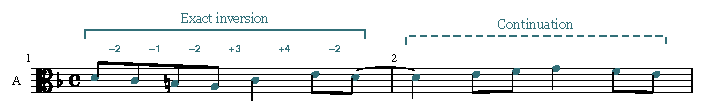
\includegraphics[width=\linewidth]{annotated/head.pdf}\par
\vspace{6mm}
{\large D minor\quad\textperiodcentered\quad 26 measures\quad\textperiodcentered\quad For one manual}\par
\vspace{5mm}
\emph{Fuga inversa} uses the exact inversion of the LICC, or Lick, the seven-note cell D--E--F--G--E--C--D. The inverted cell's harmonic meaning changes as it passes between voices. The 26-bar design moves from successive statements to overlapping imitation: the two-bar spacing of the exposition contracts to one eighth note at the tonic return. That change gives the return a different contrapuntal function. The listener encounters familiar pitches under greater temporal pressure, before the bass restores the opening subject and the final cadence brings the three voices to rest.
\vfill
{\sffamily\small Composition, analysis and production by GPT-6 Astra agents\\
Directed by chi-feng\\[5pt]7 September 2026}\par
\vspace{3mm}
{\small\href{https://chi-feng.github.io/fuga-inversa/}{Recordings, interactive score and source edition}}\par
\end{titlepage}
\setcounter{page}{1}
\section{The composition}\label{the-composition}

The score supports the designation \textbf{three-voice fugue}, with the compact scale also suggested by \emph{fughetta}. It contains a complete exposition, intervening episodes, middle entries at new pitch levels, a tonic return, and a separate cadential close. The distinction between fugue and fughetta has no dependable bar-count threshold. Prout already acknowledged its uncertainty in his nineteenth-century account, describing a fughetta as a compressed but complete composition. His terminology helps describe the scale here without making brevity a failure of form. \href{https://en.wikisource.org/wiki/Fugue_(Prout)/Chapter_10}{Prout, \emph{Fugue}, §§350--353}.

\section{Subject and answer}\label{subject-and-answer}

The commission asked for ``a 3-part fugue using the inverted LICC in the style of Bach, arranged for single manual.'' Here LICC refers to the Lick, stated on D as D--E--F--G--E--C--D. Its successive semitone intervals are +2, +1, +2, −3, −4, +2. Reversing each direction while retaining its size produces D--C--B♮--A--C--E--D: −2, −1, −2, +3, +4, −2. This is the exact inversion used in the score. Substituting B♭ would change two intervals and remove the defining chromatic constraint.

\begin{figure}[!htbp]
\centering
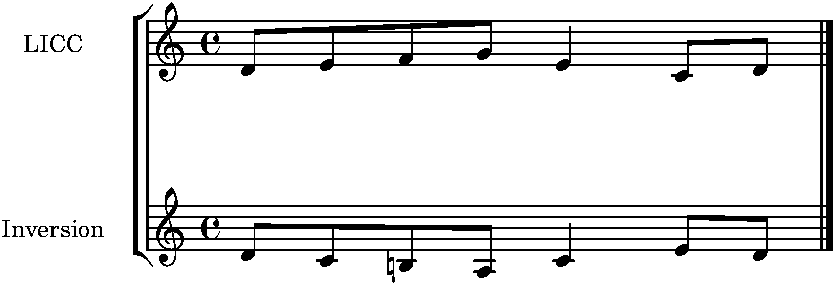
\includegraphics[width=.83\linewidth]{../assets/score/licc-reference.pdf}
\caption*{\textbf{The LICC and its inversion.} The original cell and its reflection about D share the same rhythm. Each directed interval changes sign.}
\end{figure}

The alto presents this cell alone in m.~1. Four eighth notes descend through a perfect fourth, D4--C4--B3--A3. The quarter-note C4 arrests that descent, and two eighth notes, E4--D4, close the bar. The last D is tied into m.~2. Its continuation rises through E4--F4 to G4, then descends F4--E4. The complete two-bar presentation spans a minor seventh, A3--G4, and ends on the supertonic. That open ending makes the next entry feel continuous with the first statement.

\begin{figure}[!htbp]
\centering
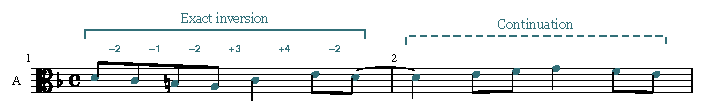
\includegraphics[width=\linewidth]{annotated/head.pdf}
\caption{Alto, mm.~1--2. The bracketed head preserves every directed semitone interval of the inversion. The continuation supplies F♮ and ends on E; the tie carries the final head note across the bar line.}
\label{ex01-subject}
\end{figure}

The head omits the third of its local scale, leaving its mode open. The F♮ of the continuation completes a Dorian collection, while later cadences establish the piece's functional D-minor setting. The opening thus combines a modal inflection in the melody with a tonal course established over the following bars.

The soprano answer in m.~3 transposes all seven head notes up a perfect fifth: A4--G4--F♯4--E4--G4--B4--A4. Its continuation ends on A4 in m.~4, where a literal transposition of the opening continuation would end on B4. The answer is therefore real at the level of the invariant head, with an adjusted ending. The term \emph{tonal answer} would suggest a more specific tonic--dominant accommodation within the thematic intervals. The UCSB account illustrates that accommodation through Bach's C-minor fugue, BWV 847, whose opening fourth changes to a fifth in the answer. Here the head's intervals remain intact. \href{https://rothfarb.faculty.music.ucsb.edu/courses/103/subject_answer.pdf}{UCSB, ``Fugue: Subject and Tonal Answer''}.

The bass enters in m.~5 with the opening subject an octave below the alto's original statement. Its m.~6 continuation is also literal. The exposition thus establishes a flexible thematic practice through an exact first statement, an adjusted answer, and an exact tonic restatement.

\section{Counterline and form}\label{counterline-and-form}

The alto's accompaniment to the answer introduces a recurring one-bar counterline: C4--D4--C4--B3--G♯3--A3 in m.~3. The soprano transposes it up a fourth in m.~5, giving F4--G4--F4--E4--C♯4--D4. Its opening quarter note allows the subject's first two eighth notes to register against a held tone. Its concluding leading-tone motion supplies the C♯--D that the D-based head itself lacks.

This counterline performs a countersubject's role beside the head, while its continuation remains flexible. It returns in the alto at m.~9 and the soprano at mm.~11, 15, and 21. The C-major version, E5--F5--E5--D5--B4--C5, changes the quality of the opening step to fit the major mode. The distinction is audible and analytical: the subject head preserves chromatic intervals, while the counterline preserves a tonal pattern through modal adjustment.

\begin{figure}[!htbp]
\centering
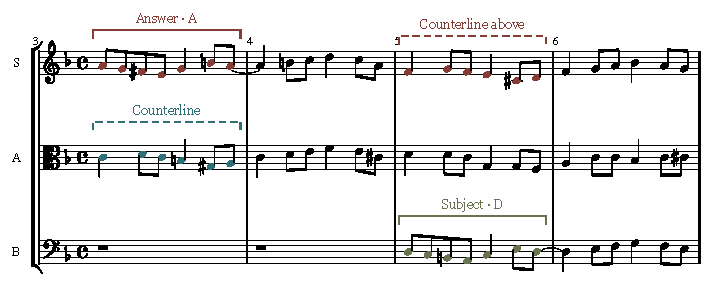
\includegraphics[width=\linewidth]{annotated/exposition.pdf}
\caption{Mm. 3--6. The first-bar subject and counterline exchange positions at the fifteenth. The consonant fifth at m.~3, beat 1½, becomes a correctly treated passing fourth in m.~5.}
\label{ex02-exposition}
\end{figure}

The first-bar pair demonstrates invertible counterpoint at the fifteenth. Transposing both m.~3 voices up a fourth, then lowering the subject by two octaves, produces the bass subject and soprano counterline of m.~5 exactly. This exchanges the positions of two lines, a different operation from the melodic inversion that produced the subject. It also changes one interval's function: G4 above C4 at m.~3, beat 1½, is a consonant fifth; the corresponding F4 above C3 in m.~5 is a compound fourth, made permissible by the weak passing bass C3 between D3 and B2. The claim is limited to the first-bar combination. The two-bar continuations are not literal derivatives.

Bach's BWV 847 offers a useful comparison: Hutchinson's annotated score tracks a recurring countersubject between voices and identifies fragments of both subject and counterpoint in episodes. \emph{Fuga inversa} uses these resources on a smaller scale, with a less stable continuation and one principal ornamental episode figure. \href{https://musictheory.pugetsound.edu/mt21c/FugueAnalysis.html}{Hutchinson, §30.8}.

{\def\LTcaptype{table}
\par\addvspace{\LTpre}
{\small\noindent
\begin{tabular}{@{}
  >{\raggedright\arraybackslash}p{(\linewidth - 4\tabcolsep) * \real{0.1600}}
  >{\raggedright\arraybackslash}p{(\linewidth - 4\tabcolsep) * \real{0.2600}}
  >{\raggedright\arraybackslash}p{(\linewidth - 4\tabcolsep) * \real{0.5800}}@{}}
\toprule\noalign{}
\begin{minipage}[b]{\linewidth}\raggedright
Location
\end{minipage} & \begin{minipage}[b]{\linewidth}\raggedright
Entering voice and pitch
\end{minipage} & \begin{minipage}[b]{\linewidth}\raggedright
Thematic and tonal evidence
\end{minipage} \\
\midrule\noalign{}

Mm. 1--2 & Alto, D4 & Exact head and original continuation; F♮ establishes the minor third. \\
Mm. 3--4 & Soprano, A4 & Exact fifth-transposed head; final continuation note adjusted to A4. \\
Mm. 5--6 & Bass, D3 & Complete opening subject transposed down an octave. \\
Mm. 9--10 & Soprano, G4 & Exact head after D-major harmony; B♭ supports a local G-minor region. \\
Mm. 11--12 & Alto, C4 & Exact C-based head with B♭; E♮ in accompaniment and continuation supports C major. \\
Mm. 15--16 & Bass, F3 & Exact F-based head with E♭; A♮ supplies a major third. \\
M. 19 into m.~20 & Soprano, D5; alto, A4 one eighth later & Complete overlapping heads; both continuations recomposed. \\
Mm. 21--22 & Bass, D3 & Literal return of mm.~5--6, including both accompanying voices. \\
\bottomrule
\end{tabular}
\par}
\addvspace{\LTpost}
}

The episodes occupy mm.~7--8 and 13--14; mm.~17--18 prepare the return through suspensions and dominant harmony. Mm. 23--26 form the cadential extension.

\section{Middle entries and episodes}\label{middle-entries-and-episodes}

The first episode changes the rhythmic surface without losing contact with the established material. Each quarter-note beat in m.~7 begins with an eighth note and ends with two sixteenths: F4--E4--F4, G4--F4--G4, E4--D4--E4, F4--E4--F4. The neighboring motion recalls the counterline's F--G--F turn, but there is no literal diminution of the complete subject. The connection lies in shared stepwise material given a new rhythmic profile.

Its bass, D3--G2--C3--F2, makes the sequence's descending-fifth relations clear. In m.~8, B♭2--G2--A2--D3 redirects that motion. The last two quarter-note harmonies are A major and D major. F♯4 then rises to G4 over the bass D3--G2 at the m.~9 entry, giving specific evidence for the G-minor arrival.

\begin{figure}[!htbp]
\centering
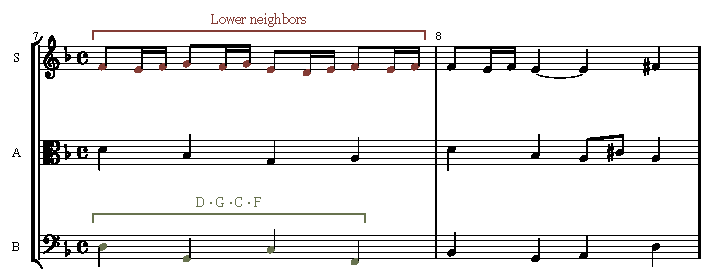
\includegraphics[width=\linewidth]{annotated/episode-one.pdf}
\caption{Mm. 7--8. Lower-neighbor sixteenths animate the soprano above the bass sequence. The final A-major and D-major sonorities prepare the G-based entry. The tied E4 in m.~8 remains consonant against the bass.}
\label{ex03-first-episode}
\end{figure}

D--G--C--F--D names the principal entry centers; their tonal weight is unequal. The G-minor arrival has a direct dominant--tonic approach. C major emerges through G/B to C in the final eighth-note motion of m.~10, then receives E♮ above its m.~11 head and within its continuation. F major receives C-major preparation at the end of m.~14 and A♮ at the m.~15 arrival. These are brief local regions within a strongly directed return to D. The score gives less evidence for prolonged, independent key areas.

The major-mode entries reveal the value of separating the invariant head from its harmony. In m.~11, beat 3, the actual sonority is G3--B♭3--D5, a G-minor triad. Beat 4 replaces it with G3--D4--B4, a G-major triad, before C/E arrives on the following eighth. The subject's B♭ and the counterline's B♮ therefore have different jobs within the same local C-major phrase. At m.~15, beat 3, E♭3--B♭3--G4 similarly gives E♭ major within the F-directed statement. E♮ appears in the following E-diminished triad over G and resolves to F.

\begin{figure}[!htbp]
\centering
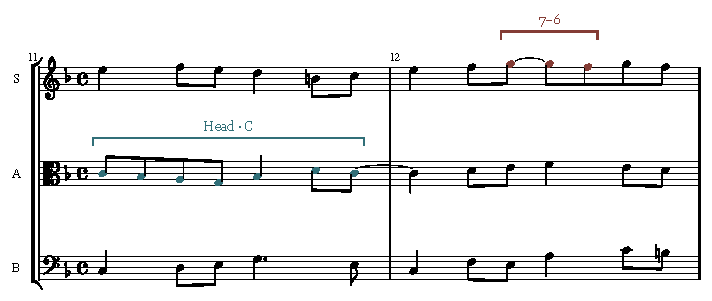
\includegraphics[width=\linewidth]{annotated/c-entry.pdf}
\caption{Mm. 11--12. The C-based head retains B♭, while the surrounding voices establish a major-mode context. G minor becomes G major in m.~11; the following bar contains a prepared G5--F5 suspension.}
\label{ex04-c-entry}
\end{figure}

The second episode transfers the sixteenth-note figure to the alto. Its quarter-note framework in mm.~13--14 is G4--A4--F4--G4, then E4--F4--D4--E4. The soprano now provides the slower line. This exchange makes the middle voice carry an idea previously associated with the top voice, while the two-bar bass sequence expands the earlier episode's harmonic travel.

The bass roots are C--F--B♭--E♭--A--D--G--C. Most adjacent roots follow descending-fifth relations, with a tritone link from E♭ to A. The sequence also changes chord quality: the E♭-major sonority gives way to A minor, whose E♮ restores the pitch required for the subsequent approach to F. Calling the entire passage an exact chain of perfect fifths would conceal this adjustment. Its final C-major harmony makes the F entry intelligible without a separate connecting passage.

\begin{figure}[!htbp]
\centering
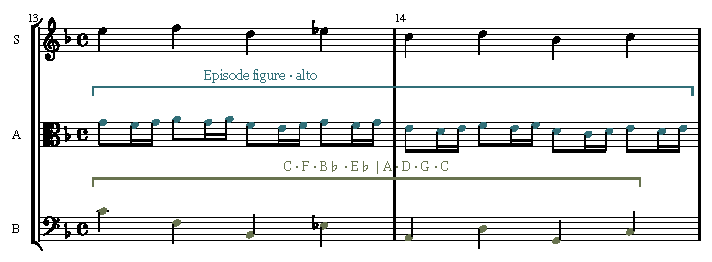
\includegraphics[width=\linewidth]{annotated/episode-two.pdf}
\caption{Mm. 13--14. The ornamental figure moves to the alto. The bass-root sequence C--F--B♭--E♭--A--D--G--C includes a tritone link and ends with C-major preparation for F.}
\label{ex05-second-episode}
\end{figure}

\section{Dissonance and preparation}\label{dissonance-and-preparation}

The score's dissonances require analysis of duration, preparation, and bass support. In m.~5, the passing bass C3 on beat 1½ places held D4 and F4 a ninth and eleventh above it, between consonant neighboring sonorities. The first E4 sixteenth of m.~7 has a different function: it is a lower neighbor to F4, sounding against D3 and D4 before returning to F4. These labels follow from the surrounding voices as well as the melodic contour.

Suspensions hold a previously consonant pitch into a dissonant position and resolve it downward by step. The numerical label depends on the interval against the bass at the dissonance and resolution. \href{https://musictheory.pugetsound.edu/mt21c/Suspension.html}{Hutchinson, §10.9}.

{\def\LTcaptype{table}
\par\addvspace{\LTpre}
{\small\noindent
\begin{tabular}{@{}
  >{\raggedright\arraybackslash}p{(\linewidth - 4\tabcolsep) * \real{0.2000}}
  >{\raggedright\arraybackslash}p{(\linewidth - 4\tabcolsep) * \real{0.2400}}
  >{\raggedright\arraybackslash}p{(\linewidth - 4\tabcolsep) * \real{0.5600}}@{}}
\toprule\noalign{}
\begin{minipage}[b]{\linewidth}\raggedright
Location
\end{minipage} & \begin{minipage}[b]{\linewidth}\raggedright
Preparation
\end{minipage} & \begin{minipage}[b]{\linewidth}\raggedright
Dissonance and resolution
\end{minipage} \\
\midrule\noalign{}

M. 12, beats 2½--3½ & Soprano G5 over bass E3 & G5 is held over A3 at beat 3, then resolves to F5: \textbf{7--6} against the bass, with \textbf{9--8} against alto F4. The resolution doubles F at the octave. \\
M. 17, beats 1--2½ & Soprano A4 over F3 & A4 is held over B♭2 at beat 2, then falls to G4: \textbf{7--6}. Alto D4 remains in place. \\
M. 18, beats 1--2½ & Soprano F4 over D3 & F4 is held over E3 at beat 2, then falls to E4: \textbf{9--8}. The alto moves G3--B3 over the same bass. \\
\bottomrule
\end{tabular}
\par}
\addvspace{\LTpost}
}

The m.~12 resolution doubles the root of F/A, locally IV6 in C. Its upper-part 9--8 departs from the restriction in Gran's strict species framework, a narrower convention than the tonal voice leading assessed here. \href{https://mtosmt.org/issues/mto.24.30.2/mto.24.30.2.gran.html}{Gran 2024, §3.7}.

The sustained G4 later in m.~17 needs a different description. It becomes the prepared seventh of A7 when the bass reaches A2 and the alto C♯4. Its resolution to F4 occurs over a new D3 bass in m.~18. That changing support makes it a prepared dominant seventh, rather than the stationary-bass 7--6 configuration just heard earlier in the bar.

The tied E4 in m.~8 supplies a useful counterexample: it is a sixth above G2 and a fifth above A2. The tie creates rhythmic continuity without creating a suspension against the bass. Likewise, the C♯4--G3 tritone over E3 in m.~5 is part of a first-inversion leading-tone triad. C♯ rises to D, G falls to F, and the bass E falls to D on the following eighth. Its dissonance has harmonic function and a specific resolution.

\begin{figure}[!htbp]
\centering
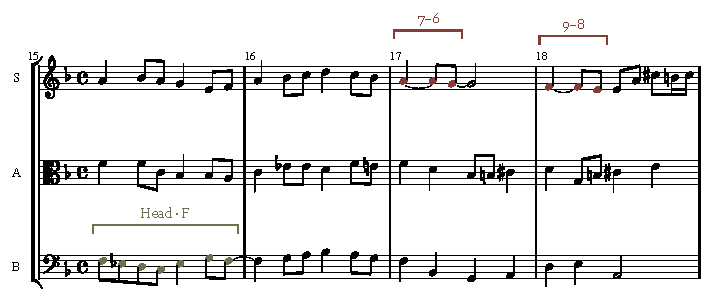
\includegraphics[width=\linewidth]{annotated/suspensions.pdf}
\caption{Mm. 15--18. The F-based entry combines an invariant E♭ with major-mode A♮. The following preparation contains a 7--6 suspension over B♭, a prepared dominant seventh, and a 9--8 suspension over E. These labels refer to different events.}
\label{ex06-f-entry-preparation}
\end{figure}

\section{The tonic return}\label{the-tonic-return}

The return in mm.~19--20 compresses the exposition's imitative spacing from two bars to one eighth note. The soprano begins D5--C5--B4--A4--C5--E5--D5 on the downbeat. The alto follows on A4 at beat 1½ with A4--G4--F♯4--E4--G4--B4--A4. The interval of entrance is a perfect fourth below the soprano; the time delay is one eighth note. These are separate quantities. The alto's A starting pitch specifies the imitative relationship, while the accompaniment gives no sustained establishment of A as a local tonic.

Both seven-note heads are complete. Their continuations change, so the passage is a stretto of the invariant cell, not a literal two-bar canon. At m.~20 the soprano descends D5--B♭4--A4--G4, while the alto completes its head and then continues G4--F4--E4--D4--C♯4. The familiar counterline has yielded its place to another thematic entry. After this concentration, its return above the bass subject in m.~21 restores the exposition's more spacious relationship.

\begin{figure}[!htbp]
\centering
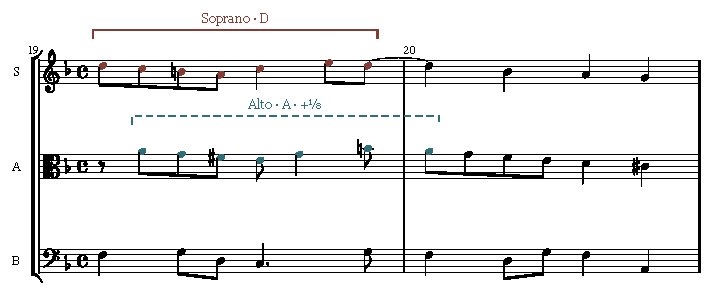
\includegraphics[width=\linewidth]{annotated/return.pdf}
\caption{Mm. 19--20. Brackets identify two exact heads separated by one eighth note. The bass supports both upper fourths. The continuations diverge before the complete three-voice return of mm.~5--6 begins at m.~21.}
\label{ex07-return}
\end{figure}

{\def\LTcaptype{table}
\par\addvspace{\LTpre}
{\small\noindent
\begin{tabular}{@{}
  >{\raggedright\arraybackslash}p{(\linewidth - 8\tabcolsep) * \real{0.1900}}
  >{\raggedright\arraybackslash}p{(\linewidth - 8\tabcolsep) * \real{0.1200}}
  >{\raggedright\arraybackslash}p{(\linewidth - 8\tabcolsep) * \real{0.1200}}
  >{\raggedright\arraybackslash}p{(\linewidth - 8\tabcolsep) * \real{0.1200}}
  >{\raggedright\arraybackslash}p{(\linewidth - 8\tabcolsep) * \real{0.4500}}@{}}
\toprule\noalign{}
\begin{minipage}[b]{\linewidth}\raggedright
Time
\end{minipage} & \begin{minipage}[b]{\linewidth}\raggedright
Soprano
\end{minipage} & \begin{minipage}[b]{\linewidth}\raggedright
Alto
\end{minipage} & \begin{minipage}[b]{\linewidth}\raggedright
Bass
\end{minipage} & \begin{minipage}[b]{\linewidth}\raggedright
Sonority or contrapuntal function
\end{minipage} \\
\midrule\noalign{}

M. 19, beat 1 & D5 & Rest & F3 & Incomplete D-minor tonic in first inversion. \\
Beat 1½ & C5 & A4 & F3 & F major; alto head begins. \\
Beat 2 & B4 & G4 & G3 & G major without its fifth. \\
Beat 2½ & A4 & F♯4 & D3 & D major; F♯ subsequently descends to E. \\
Beat 3 & C5 & E4 & C3 & C major without its fifth. \\
Beat 3½ & C5 & G4 & C3 & Upper fourth supported by fifth and octave above C. \\
Beat 4 & E5 & G4 & C3 & Complete C-major triad. \\
Beat 4½ & D5 & B4 & G3 & Complete G-major triad. \\
M. 20, beat 1 & D5 & A4 & F3 & Upper fourth supported by third and sixth above F. \\
\bottomrule
\end{tabular}
\par}
\addvspace{\LTpost}
}

The fourths in this table are supported consonances: each upper note is consonant against the bass. Gran's account of three-voice canonic writing distinguishes this case from a fourth formed with the lowest voice. \href{https://mtosmt.org/issues/mto.24.30.2/mto.24.30.2.gran.html}{Gran 2024, §§3.7--3.8}. At m.~20, beat 1½, the alto G4 is a dissonant ninth above F3. It passes downward between A4 and F4 on a weak eighth note.

The D-major chord in m.~19 is followed by C major, with F♯4 falling to E4. A reading that treats F♯ as a leading tone resolving to G would contradict the written line. The harmonic succession accommodates the exact overlapping heads through changing consonant support. The tonic return has two stages: thematic D returns over F in m.~19; root-position D and the original accompaniment return in m.~21 after A7. The second arrival consolidates a tonic that the overlapping heads have already recalled.

\section{Cadence and keyboard writing}\label{cadence-and-keyboard-writing}

The cadential extension broadens the rhythm. In the second half of m.~24, G2--B♭3--E♭4 forms E♭ major in first inversion, the Neapolitan sixth of D minor. Its placement before the dominant, and its bass on scale degree 4, establish the function. The next bar gives A2--F3--D4, then A2--E3--C♯4: cadential six-four to dominant. The soprano E♭--D--C♯ traces ♭2--1--7, the intervening tonic delaying arrival at the leading tone. The line follows the Neapolitan's usual downward resolution, here accommodated by the six-four. \href{https://musictheory.pugetsound.edu/mt21c/VoiceLeadingNeapolitanChord.html}{Hutchinson, §29.3, fig.~29.3.1}.

The six-four has dominant function here: its D and F resolve to C♯ and E above the held A bass. \href{https://musictheory.pugetsound.edu/mt21c/TheCadentialSixFourChord.html}{Hutchinson, §16.3}. The alto's complete approach is B♭3--F3--E3. Its descending fourth into the six-four changes register at a point where soprano and bass move by step. This leap is the score's particular voicing choice; the subsequent F3--E3 supplies its stepwise resolution.

\begin{figure}[!htbp]
\centering
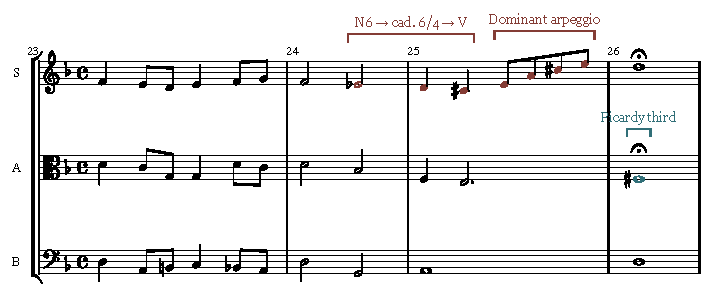
\includegraphics[width=\linewidth]{annotated/coda.pdf}
\caption{Mm. 23--26. N6 proceeds through a cadential six-four to V and the final major tonic. The soprano traces E♭4--D4--C♯4, and the alto resolves F3--E3. The right hand plays the arpeggio while the left sustains bass and alto.}
\label{ex08-cadence}
\end{figure}

The final arpeggio E4--A4--C♯5--E5 prolongs the dominant and returns the soprano to a higher register, below the G5 peak reached in m.~12. The final D5 above D3 and F♯3 gives a Picardy-third close with the fifth omitted. Its force comes from the preceding dominant duration, the soprano's descent E5--D5, the bass A2--D3, and the broad final note values.

The single-manual requirement is met through hand redistribution. Voice identity persists when the alto changes staff. At mm.~11--12 the left hand takes bass and alto while the soprano occupies the higher register. At mm.~25--26 the same division allows the right hand's arpeggio above sustained lower notes. Reading soprano and alto as an inseparable right-hand pair would invent a two-octave stretch at the end that the printed allocation avoids. The written ranges are soprano C♯4--G5, alto E3--B4, and bass F2--C4. Instantaneous spans are compatible with an octave hand; fluent legato still depends on fingering and timely transfers.

\section{Scale and limitations}\label{scale-and-limitations}

The piece's strongest formal contrast is the change from successive entries to the late compressed overlap. The transfer of the episode figure and the distinction between exact head and flexible tonal counterline prepare that contrast. The resulting unity has clear limits. The continuation is less memorable and less consistently retained than the head. Both main episodes rely on closely related neighbor figures and descending-fifth procedures. Local key areas receive only brief confirmation, and the stretto supplies a single concentrated test of the head's contrapuntal potential.

Those limits support the description of a compact fugue or fughetta. They also set a boundary on the Bach comparison. The score uses thematic recurrence, functional bass motion, controlled suspensions, and a late increase in imitative density. It does not demonstrate the broader network of sustained canons, multiple countersubjects, or thematic transformations found across Bach's output. Such devices are not a checklist for an individual fugue. Here their limited presence means that the final cadence closes a concise exploration of one cell, with the return's changed temporal relation carrying most of the formal argument.

\section{Sources and score reference}\label{sources-and-score-reference}

Pitch names use scientific pitch notation, with middle C designated C4. Half-beat references identify eighth-note positions in 4/4. Musical claims above refer to the final 26-bar source, including the two-entry stretto in mm.~19--20 and the arpeggiated close in mm.~25--26. The note evidence was checked against the LilyPond source and the corresponding exported MIDI; the MIDI cannot establish note spelling or the harmonic meaning of an interval.

\begin{itemize}
\tightlist
\item
  \textbf{Score:} GPT-6 Astra. 2026. \emph{Fuga inversa}, for a single manual, in three voices. \href{https://chi-feng.github.io/fuga-inversa/assets/score/fugue.ly}{LilyPond source}. The accompanying \href{https://chi-feng.github.io/fuga-inversa/assets/evidence/excerpt-specifications.json}{excerpt and evidence file} records the source and MIDI hashes for this edition.
\item
  \textbf{Gran, Jacob.} 2024. ``A General Method for Composing a Canon Against a Cantus Firmus Using Sergei Taneev's Double-Shifting Counterpoint.'' \emph{Music Theory Online} 30 (2), June. \href{https://mtosmt.org/issues/mto.24.30.2/mto.24.30.2.gran.html}{Article and examples}. DOI: 10.30535/mto.30.2.4, especially §§3.7--3.8.
\item
  \textbf{Hutchinson, Robert.} \emph{Music Theory for the 21st-Century Classroom}. Website copyright 2017. \href{https://musictheory.pugetsound.edu/mt21c/Suspension.html}{§10.9, ``Suspension''}; \href{https://musictheory.pugetsound.edu/mt21c/TheCadentialSixFourChord.html}{§16.3, ``The Cadential Six-Four Chord''}; \href{https://musictheory.pugetsound.edu/mt21c/VoiceLeadingNeapolitanChord.html}{§29.3, ``Voice Leading the Neapolitan Chord''}; \href{https://musictheory.pugetsound.edu/mt21c/FugueAnalysis.html}{§30.8, ``Fugue Analysis''}. The BWV 847 comparison refers to the score examples and commentary in §30.8.
\item
  \textbf{Prout, Ebenezer.} 1891. \emph{Fugue}, chapter 10, ``Fughetta and Fugato,'' especially §§350--353. \href{https://en.wikisource.org/wiki/Fugue_(Prout)/Chapter_10}{Public-domain text}.
\item
  \textbf{University of California, Santa Barbara.} ``Fugue: Subject and Tonal Answer.'' Undated course handout hosted on Lee Rothfarb's faculty site. \href{https://rothfarb.faculty.music.ucsb.edu/courses/103/subject_answer.pdf}{Two-page PDF}.
\end{itemize}

External sources consulted 7 September 2026. The original score analysis, pitch tables, and evaluations are specific to \emph{Fuga inversa}.

\clearpage

\section{Appendix}\label{appendix}

\subsection{Process and evaluation}\label{process-and-evaluation}

This appendix records how the 26-bar \emph{Fuga inversa} was composed, revised, and checked. The final score derives from candidate C, with a later stretto, a revised closing register, and explicit transfers of the middle voice between hands. The evidence consists of the LilyPond sources, compiled MIDI files, saved audit reports, candidate reviews, and performance scripts. The project records describe work undertaken on 7 September 2026.

\subsection{Musical constraint and proposals}\label{musical-constraint-and-proposals}

The user approved an exact inversion of the seven-note Lick, D--E--F--G--E--C--D. Reflection about its initial D gives D--C--B-natural--A--C--E--D. Its directed semitone intervals are −2, −1, −2, +3, +4, −2. The rhythm remains four eighth notes, a quarter note, and two eighth notes; the last note can be tied into the following bar. A diatonic adjustment from B-natural to B-flat would change the required interval sequence. This distinction affected the harmony throughout the composition.

The compositional working brief specified three monophonic voices on one organ manual, a literal tonic--dominant--tonic exposition, recurring counterpoint, episodes, and a credible return and cadence. The dominant answer therefore transposes the complete cell to A--G--F-sharp--E--G--B--A. Harmonic adjustments belong in the accompanying voices or continuation, while the recurring seven-note cell retains its pitches and rhythm under transposition.

At the user's request, three GPT-6 Astra composing agents worked at maximum reasoning effort. Each produced a separate candidate, compiled a score, and supplied notes for review. Their initial proposals were separate assignments, but the later revisions shared a brief, an auditor, coordinator feedback, and cross-reviews. This was a comparison of compositions produced under a common method.

The recommendation was not unanimous. A and C recommended B. Both valued B's recurring two-bar countermelody, high-register entry, and clear rise and return. B recommended C because its episodes move between voices and its middle section travels through G, C, and F. The coordinator retained C. C's own review identified its regular phrase lengths and frequent parallel thirds and sixths as limitations relative to B. That objection remains relevant to the comparison; passing an interval audit does not settle it. The reviews also predate the final stretto and expanded closing register, so they should not be presented as votes on the finished version.

\subsection{Revisions that changed the score}\label{revisions-that-changed-the-score}

The saved reports contain failures as well as successful revisions. An early A audit found parallel octaves in bar 6: soprano C-sharp5--D5 above bass C-sharp3--D3, from the second half of beat 2 to beat 3. Later A files contain revised notes. These snapshots establish a correction history; they do not show that the present A source still contains those octaves.

C's first saved audit covered only ten bars. Its adjacent-event scan found no perfect-interval flag, yet bar 10 contained two problems. On the quarter-note grid, alto C4 above bass F2 moved to E4 above A2, producing successive fifths. The intervening eighth-note sonority prompted a review of the underlying motion. At beat 4, G2--B3--D5 also exceeded the intended hand reach: either adjacent pair required more than an octave. The final version revises both the approach and the sonority, reaching B2--G4--D5 at that beat. The upper pair then fits comfortably within an octave. Unequal draft lengths make the first audit reports unsuitable for ranking the agents by failure count.

The closing revision changes musical direction without adding a voice. The final soprano reads:

\begin{verbatim}
d'4 cis'4 e'8 a'8 cis''8 e''8 | d''1
\end{verbatim}

The line rises through the dominant arpeggio to the final D5. Below it, F3 moves to E3 over A2 in bar 25, then to F-sharp3 over D3 in bar 26. The cadential six-four resolves before the arpeggio; the final chord contains exactly D3, F-sharp3, and D5. The wider register therefore comes from a single melodic line and an open three-note ending.

A later request for greater ambition led to a separate stretto study. The earlier C review correctly stated that its version contained no stretto. The new study tested a D entry in the soprano against a complete A answer beginning one eighth note later in the alto. Both heads retain the prescribed intervals and rhythm. They overlap for the remaining three and a half beats of bar 19, with the alto's final A4 falling on the first eighth of bar 20.

The study included unchanged bars 18 and 21 so that the approach and exit could be examined. It was engraved, compiled, and audited before the coordinator adopted its replacement for bars 19--20. The complete score was then compiled and audited again. This adds a ninth literal head within the existing 26 bars. The return now layers a tonic subject and dominant answer over an independent bass.

One harmonic qualification matters. The alto's F-sharp4 on the second half of beat 2 in bar 19 belongs to the exact G4--F-sharp4--E4 descent. It is consonant above D3, and the next sonority is C major. The D-major sonority colors the line; it does not produce a dominant resolution into G. A modal and linear reading is therefore more precise than an unqualified ``V of G'' label.

\subsection{What the audit tests}\label{what-the-audit-tests}

The auditor uses the actual LilyPond MIDI as its input. It groups notes by MIDI track and channel, checks monophony and crossings, and examines every voice pair at successive note events. It flags successive perfect fifths and octaves, distinguishes similar from contrary motion, and reports direct outer perfect intervals when the upper voice leaps by more than a whole tone. A second pass samples quarter-note positions. The two resolutions caught different problems in the drafts.

The final report identifies three monophonic voices and nine literal heads, with no flags from either perfect-interval pass and no crossings. In every three-note sonority, at least one adjacent pitch pair lies within an octave; the remaining note can go to the other hand. These results apply to the compiled symbolic MIDI identified by the report's SHA-256 digest. They do not prove the absence of every objection a contrapuntal analyst could raise. A quarter-note grid is only one possible reduction; it cannot determine which notes carry harmonic weight across a longer phrase.

The subject matcher checks directed pitch intervals and relative attack times: 0, ½, 1, 1½, 2, 3, and 3½ quarter-note units. It does not independently establish every written duration or tie. Those require source inspection. MIDI also loses enharmonic spelling. The auditor cannot decide whether a pitch functions as a suspension, chord member, modal inflection, or harmonic goal.

Dissonance reports were therefore reviewed against the score. In bar 17, for example, the soprano A4 is prepared over F3, held while the bass moves to B-flat2, and resolved to G4 halfway through beat 2. The preparation and resolution explain the flagged seventh as a 7--6 suspension. Likewise, diminished sonorities need their resolutions examined. A stepwise melodic shape alone does not establish that a note is a permissible passing tone.

The auditor's fixtures include deliberate parallel fifths and octaves, a direct outer perfect interval, and examples of thirds and oblique motion that should pass. These tests passed and cover those specific program behaviors. The agents and coordinator also used the same auditor, which leaves a shared source of possible error despite their separate score readings.

\subsection{Notation and performance}\label{notation-and-performance}

The reach check asks whether one adjacent pair of the three sounding pitches can fit within an octave, leaving the other pitch to the other hand. This is an instantaneous condition. It does not supply fingering or establish that successive allocations preserve legato comfortably. The final score explicitly puts the alto in the left hand at bars 3--4, the end of bar 9, bars 11--12, and bars 25--26. At bar 9 beat 4, the low F-sharp3--G3 belongs with the left hand; at bar 11, C4 above bass C3 gives an octave. The closing F3--E3--F-sharp3 remains below the rising soprano. A separate check against the actual printed hand transfers found no simultaneous span above an octave in either hand. No live keyboard trial forms part of the evidence recorded here.

A MIDI fixture exposed a separate technical issue. LilyPond's voice channel setting still reused channel numbers across different staves. The audit could distinguish those notes by track and channel, but rendering required globally distinct voice channels. The preparation script remaps them and asserts that pitches and attack times survive. All organ voices then use the same registration. This finding concerns channel identity; it is not evidence that an audible note cutoff was heard in the candidate recordings.

The printed score and the MIDI export also serve different purposes. The printed score has two staves with hand transfers. A separate MIDI score keeps each contrapuntal voice on its own staff, preventing those printed transfers from splitting its identity. The symbolic MIDI remains the authority for interval analysis. Performance changes belong in derived files.

The organ realization uses Joseph Basquin's Jeux d'orgues 2.1 samples of the Stiehr--Mockers organ at Romanswiller. All three voices share the principal 8\textquotesingle{} + 4\textquotesingle{} registration. An 18-millisecond release gap supplies modest separation, while the tempo remains quarter note = 92 until the final bar slows to 60. The registration belongs to one manual; no pedal division is used. \href{https://www.jeuxdorgues.com/jeux-d-orgues-2-stiehr-mockers/}{Instrument and samples}.

The first piano realization used the Salamander Grand Piano SoundFont. The user found it too mechanical, despite its existing tempo, velocity, and articulation changes. That feedback prompted two separate revisions: a more pronounced interpretation and a different piano instrument. The final piano MIDI follows a smooth tempo curve, with the episodes approaching quarter note = 98--100, relaxation around the suspensions, and a broader cadential approach. The last whole note is held at quarter note = 54. The curve follows formal and harmonic events rather than random timing variation.

Note-on velocities range from 50 to 89. The entering head receives prominence even when it lies in the bass or alto; accompanying voices remain quieter. The descending head, local peaks, prepared dissonances, and resolutions have distinct attack weights. Releases vary with note length, melodic role, repetition, leap, and phrase boundary. Selected arrivals have small offsets, up to 17 milliseconds. Seven short harmonic spans use the damper pedal, with the remaining counterpoint kept clear of sustained pedal. The source and derived MIDI retain the same 382 pitches in the same order within each voice. These checks establish the interpretation's relation to the score; they do not measure its resemblance to a human pianist.

\begin{figure}[!htbp]
\centering
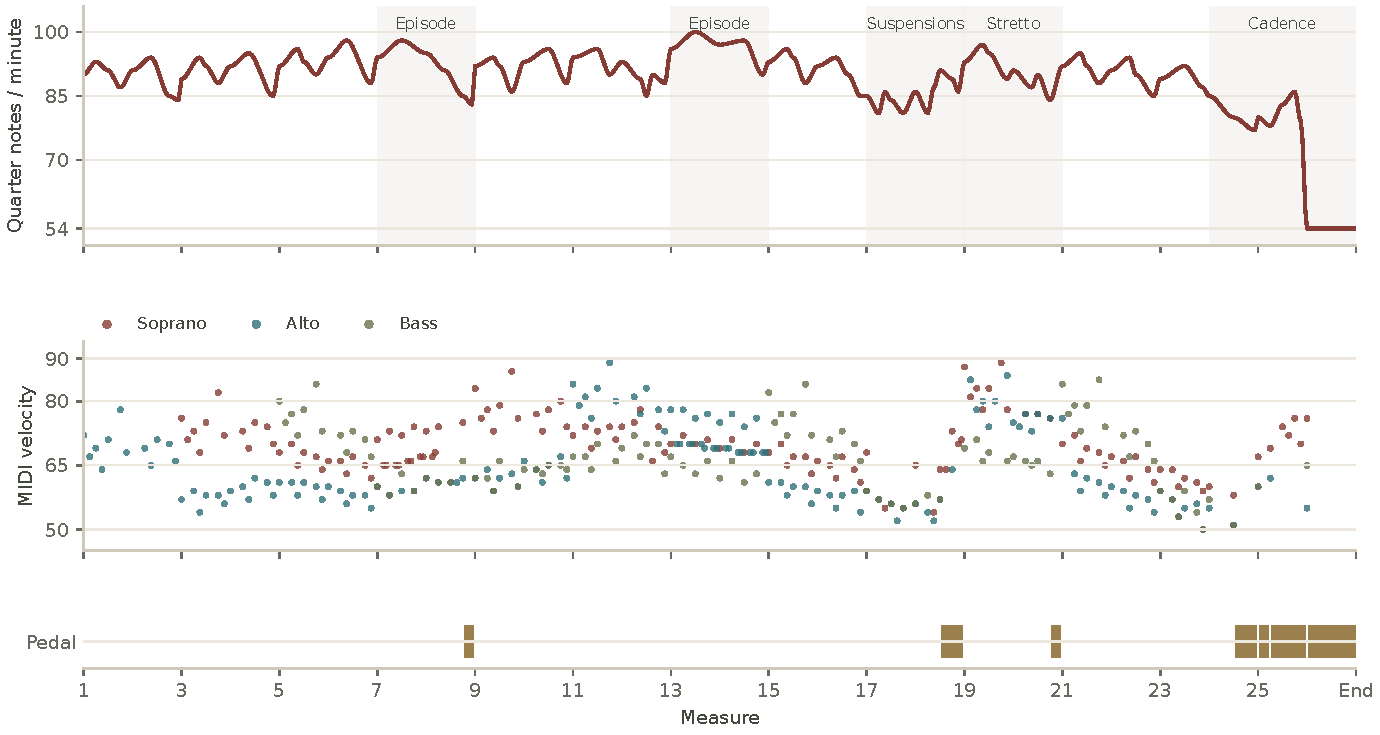
\includegraphics[width=\linewidth]{../assets/figures/piano-performance.pdf}
\caption*{\textbf{Figure A1.} The final piano MIDI's tempo, note-on velocities, and pedal spans. Velocity is a MIDI control value, not a measurement of recorded loudness.}
\end{figure}

The revised MIDI drives GarageBand's installed Steinway Grand Piano. The complete performance uses one piano track, which gives the instrument a common pedal and acoustic identity. The native export disables the patch's reverb, echo, and compressor. The full mix and three separate voices were exported at 44.1 kHz and 24-bit PCM, with automatic normalization disabled. Their frame counts and embedded tempo markers agree. Native piano-roll observations preserve all pitches and place attacks within one native tick of the imported MIDI. The native project did not provide a round-trip check of note lengths or velocities; those were checked in the imported MIDI. Separate voice renders use the same performance times and gain for analytical listening. The complete master remains the default recording; isolated voices are study aids.

The room treatment convolves a mono send with James Cadwallader's measured stereo response from Spokane Woman's Club, while retaining the original stereo piano as the direct signal. The OpenAIR metadata identifies an X/Y microphone at the rear of the hall, 24 metres from the stage source. Blending that capture with a dry piano creates a room perspective; it does not reconstruct a documented seat or a live concert. \href{https://www.openair.hosted.york.ac.uk/?page_id=659}{OpenAIR dataset}.

The processor removes the response's direct impulse, admits the measured reflections through a short fade, and filters only the room signal below 140 Hz and above 8 kHz. The retained response lasts 3.5 seconds. Its original broadband decay yields a 2.23-second T60 estimate from a fit over the −5 to −25 dB interval; this is an extrapolated acoustic measurement. The principal mix adds the room at −14 dB relative to the dry signal's RMS level, with 6 milliseconds of extra delay. A closer alternative uses −18 dB and 12 milliseconds. The alternatives are matched for integrated loudness, using static gain. No compressor or limiter is added to the piano master. The response is credited to James Cadwallader and OpenAIR under CC BY 4.0, with the processing changes identified in the edition's credits.

The initial candidate recommendations came from score and MIDI inspection. The production agents used source checks, render settings, waveform measurements, and loudness comparisons; they did not supply an auditory evaluation of the final recordings. The user's listening feedback changed the production plan. A pianist's performance of the engraved score, and a listening comparison with the rendered interpretation, would provide evidence beyond the symbolic checks recorded here.

\subsection{Digital edition}\label{digital-edition}

The musical examples are regenerated from the authoritative LilyPond source. A strict parser retains pitches, spellings, durations, rests, and ties; each compiled excerpt is compared with the corresponding full-score MIDI range. LilyPond 2.26's SVG output attaches source note identifiers to the engraving. The webpage uses those identifiers for analytical brackets, note explanations, and voice focus. It follows the selected recording through a time map that retains tempo changes within a beat. The organ and piano can therefore switch at the same score position.

Verovio was tested as a JavaScript notation renderer, including its semantic note identifiers. The final edition uses LilyPond SVG because the performing score was already authoritative and the paper needed short excerpts with matching printed figures. This choice preserves one engraving source. It gives up live musical reflow: phone readers scroll the fixed excerpts horizontally. The PDF uses the same annotated vector figures, typeset with XeLaTeX. \href{https://lilypond.org/doc/v2.26/Documentation/notation/alternative-output-formats}{LilyPond SVG output}, \href{https://book.verovio.org/interactive-notation/css-and-svg.html}{Verovio semantic SVG}.

\subsection{Primary artifacts}\label{primary-artifacts}

Paths are relative to the edition's \href{https://chi-feng.github.io/fuga-inversa/reproducibility/README.md}{reproducibility directory}. The first-draft MIDI files were not retained; their saved reports preserve historical findings without making those drafts rebuildable.

{\def\LTcaptype{table}
\par\addvspace{\LTpre}
{\small\noindent
\begin{tabular}{@{}
  >{\raggedright\arraybackslash}p{(\linewidth - 2\tabcolsep) * \real{0.5200}}
  >{\raggedright\arraybackslash}p{(\linewidth - 2\tabcolsep) * \real{0.4800}}@{}}
\toprule\noalign{}
\begin{minipage}[b]{\linewidth}\raggedright
Artifact
\end{minipage} & \begin{minipage}[b]{\linewidth}\raggedright
Evidence
\end{minipage} \\
\midrule\noalign{}

\nolinkurl{fugue.ly}; \nolinkurl{fugue.midi}; \nolinkurl{reports/final-audit.json} & Final notation, compiled notes, and interval findings tied to a MIDI digest \\
\nolinkurl{candidate-a/NOTES.md}; \nolinkurl{candidate-b/candidate-notes.json}; \nolinkurl{candidate-c/REVIEW.md} & Candidate forms, limitations, and differing recommendations \\
\nolinkurl{history/index.json}; \nolinkurl{history/candidate-*-*-audit.json} & Saved draft findings, with retained-file limits recorded separately \\
\nolinkurl{paper-process/stretto-study.ly}; \nolinkurl{paper-process/stretto-study-audit.json} & The adopted overlap with its approach and exit \\
\nolinkurl{audit_midi.py}; \nolinkurl{fixtures/channel-fixture.ly} & Check definitions and the channel example \\
\nolinkurl{check_hands.py}; \nolinkurl{reports/printed-hands.json}; \nolinkurl{fixtures/missing-alto-transfer.ly} & Printed hand allocation and a failing transfer example \\
\nolinkurl{piano-production/shape_performance.py}; \nolinkurl{piano-production/performance-checks.json} & Tempo, articulation, dynamics, pedal and the source-to-performance comparison \\
\nolinkurl{piano-production/garageband-import-checks.json} & Native pitch and onset checks, with round-trip limits stated \\
\nolinkurl{hall-production/hall.py}; \nolinkurl{hall-production/public-provenance.json} & Measured room processing, source hashes, native formats and delivery measurements \\
\bottomrule
\end{tabular}
\par}
\addvspace{\LTpost}
}

The complete file manifest accompanies this edition. The musical claims above should be read together with the checks' stated limits.

The complete performing score and recordings accompany this paper at \href{https://chi-feng.github.io/fuga-inversa/}{the online edition}. The \href{https://github.com/chi-feng/fuga-inversa}{source repository} preserves the scripts and the public revision evidence.
\end{document}
